% Este fichero es parte del Número 5 de la Revista Occam's Razor
% Revista Occam's Razor Número 5
%
% (c)  2010 The Occam's Razor Team
%
% Esta obra está bajo una licencia Reconocimiento 2.5 España de Creative
% Commons. Para ver una copia de esta licencia, visite 
% http://creativecommons.org/licenses/by/2.5/es/
% o envie una carta a Creative Commons, 171 Second Street, Suite 300, 
% San Francisco, California 94105, USA.

% Este .tex contiene el contenido del articulo
% Seccion (Dejar en blanco)
%

% Incluye imagen del artículo (Debe ser diferente del Kokopelli! (°_°) Sin embargo, no es obligatoria esta imagen)

%\rput(2.5,-2.3){\resizebox{!}{3.2cm}{{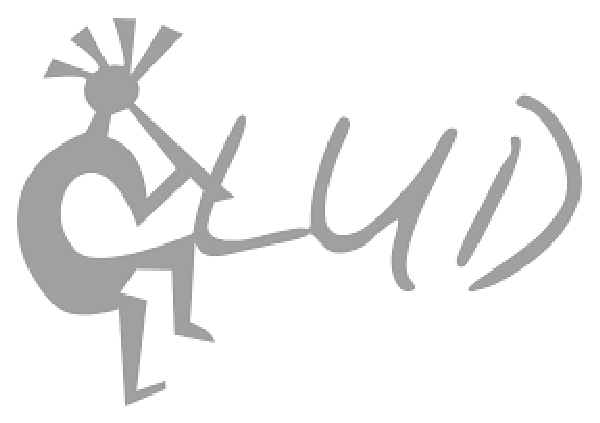
\includegraphics[]{images/nombre_articulo/glud}}}}


%Imagen de el comienzo de el articulo, coordenadas desde %la parte superior izquierda del margen de la pagina
% Las imagenes quedan mejor en formato .eps, agradecería si alguien logra colocar imagenes en dicho formato y comparte la corrección.

% -------------------------------------------------
% Cabecera
\begin{flushright}
\msection{introcolor}{black}{0.35}{Accesibilidad de plataformas}

\mtitle{10cm}{El aporte del software libre a la accesibilidad en plataformas tecnológicas.}

\msubtitle{8cm}{The contribution of free software to accessibility in technology platforms.}

{\sf Jesús David Romero, Estudiante de Ingeniería de Sistemas }

{\psset{linecolor=black,linestyle=dotted}\psline(-12,0)}
\end{flushright}

\vspace{2mm}
% -------------------------------------------------

\begin{multicols}{2}

\sectiontext{white}{black}{Resumen}

% Introducción
\intro{introcolor}{E}{ste trabajo hace un estado de arte sobre los avances en el software libre, centrándose en las herramientas que contribuyen a la accesibilidad de las plataformas tecnológicas. 
}

\sectiontext{white}{black}{Palabras clave: } Software libre, accesibilidad, plataformas tecnológicas, avance, discapacidad.


\sectiontext{white}{black}{Introducción}

La accesibilidad es una tendencia que pretende brindarle a las personas que presenten algún tipo de discapacidad, ya sea visual, auditiva o cognitiva una experiencia parcialmente completa a los contenidos audiovisuales presentes en las diferentes plataformas tecnológicas, aliado a la ideología emanada por el software libre las oportunidades de avance que hay en este campo son tan limitadas como la imaginación de los colaboradores, y la oportunidad de generar cada vez mayor inmersión en estos contenidos creando una equidad en el mundo de las tecnologías.
 
\noindent

\sectiontext{white}{black}{Accesibilidad en las tecnologías de la información}

La accesibilidad se basa en el diseño de producto y entornos de fácil uso para el mayor número de personas, enfocandose a la población más vulnerable en cuanto al uso de herramientas se refiere. Existen siete principios que apuntan al tema de la accesibilidad: la igualdad de uso, la flexibilidad, diseño simple e intuitivo, información perceptible, diseño tolerante a errores, diseño con escaso esfuerzo físico y tamaño y espacio para el acceso y uso.

Específicamente la WGAC tiene tres principios: Debe ser perceptible, operable, robusto.

La accesibilidad recoge varias clases de discapacidades: visual, cognitiva, auditiva y neurológica. Recoge también a personas que no poseen ningún tipo de discapacidad pero que por alguna condición no pueden disfrutar por completo su experiencia en la web (por ejemplo, la conexión lenta, computadores de bajos recursos, pérdida momentánea de un brazo, edad avanzada).

La W3C define accesibilidad como: \textit{"Acceso de todos a la Web, independientemente del tipo de hardware, software, infraestructura de red, idioma, cultura, localización geográfica y capacidades de los usuarios"}.


\sectiontext{white}{black}{Software Libre}

\begin{quote}
\raggedleft
“ Enseñar a los niños el uso del software libre en las escuelas, formará individuos con sentido de libertad. "\\
 Richard Stallman

\end{quote}

El software libre es el software que respeta la libertad de los usuarios y de la comunidad, en otras palabras es el derecho y la libertad que tienen los usuarios de ejecutar, copiar, distribuir, estudiar, modificar y mejorar el software; entendiendo así el software libre como una cuestión de libertad y no de precio ya que dada su escritura en ingles da para equivocaciones y malas interpretaciones.

Se dice que un software es libre cuando cumple con las siguientes 4 libertades:
\begin{itemize}
\item (Libertad 0) La libertad de ejecutar el programa como se desea, con cualquier propósito.
\item (Libertad 1) La libertad de estudiar cómo funciona el programa, y cambiarlo para que haga lo que usted quiera. El acceso al código fuente es una condición necesaria para ello.
\item (Libertad 2) La libertad de redistribuir copias para ayudar a su prójimo.
\item (Libertad 3)La libertad de distribuir copias de sus versiones modificadas a terceros. Esto le permite ofrecer a toda la comunidad la oportunidad de beneficiarse de las modificaciones. El acceso al código fuente es una condición necesaria para ello.
\end{itemize}

% Siguiente página
%%%%%%%%%%%%%%%%%%%%%%%%%%%%%%%%%%%%%%%%%%%%%%%%%%%%%%%%%%%%
\ebOpage{introcolor}{0.35}{Accesibilidad de plataformas}
%%%%%%%%%%%%%%%%%%%%%%%%%%%%%%%%%%%%%%%%%%%%%%%%%%%%%%%%%%%%


\sectiontext{white}{black}{Ventajas del Software libre}

Cuando se habla de libertad en el software libre y no se tiene profundidad en el tema, se puede quedar en el campo de la filosofía abstracta y poco práctica, por eso a continuación se esbozan algunas ventajas identificadas en el campo de la implementación de esta praxys filosófica y revolucionaria.

\begin{itemize}
\item Revisión pública: Al estar varias personas revisando sin ningún tipo de restricción el código, la detección de errores y bugs va a ser mucho más rápida.


\item Distribución de conocimientos: Aunque se es enfático en que software libre no significa software gratuito, si hay casos en que efectivamente este no presenta precio para adquirirlo, permitiendo que la adquisición de conocimientos sea mucho más dinamica y más nutrida.
\item Innovación: En el libro \textit{La catedral y el bazar} de Erick Raymond, se muestra la diferencia entre un modelo de construcción a modo catedral, hermético y vertical y un modelo bazar, variado horizontal y “bullicioso” haciendo analogía con el software privativo y el software libre respectivamente, este modelo bazar donde hay un caos constante y un ir y venir de ideas e iniciativas permite efectivamente que de todo este caos surgen constantemente mejoras y nuevos desarrollos al software inicial haciendo que la innovación esté al orden del dia.
\item Beneficio económico: Como ya se mencionó antes en efecto mucho software libre es totalmente gratuito, permitiendo que en empresas la inversión en informática no sea tan alta.
\item Seguridad: Esta ventaja va de la mano de la revisión pública pero se hace el enfásis ya que con la cantidad de datos que se manejan en la web la seguridad debe ser un indicador primordial.
\end{itemize}

\sectiontext{white}{black}{Proyectos de Software libre y accesibilidad}
\subsection*{Discapacidad visual}
\begin{itemize}
\item El proyecto Orca, para el sistema operativo Linux, combina herramientas de síntesis de voz para que el ordenador lea en voz alta lo que aparece en la pantalla, con la posibilidad de trabajar con Braille y magnificación de pantalla. Es parte de la plataforma “Gnome" de Linux. 
http://www.gnome.org/projets/orca
\item Lazaroux, este proyecto va enfocado a personas con discapacidad visual de habla hispana, es una distribución de Linux que ofrece varias herramientas y aplicaciones para facilitar la accesibilidad y un motor totalmente en castellano. No es necesaria su instalación para su utilización.
\item Mozilla Firefox, es un conocido proyecto de software libre que tiene una gran cantidad de extensiones para proporcionar accesibilidad en el contenido web.
\item Britty, es un proceso que se ejecuta en segundo plano y permite la entrada de teclados braille para usarlos en consolas de texto de Linux y Unix.
\item Festival, es un sintetizador de voces, disponible en inglés y en español para diferentes distribuciones. Con documentación completa para la implementación de nuevas voces.
\item Gnome-Speech, es una libreria API general que permite la programación de software basado en Gnome para producir voz, actualmente solo está disponible la interfaz de Festival.
\item Gnopernicus, brinda a los usuarios con discapacidad visual o visión limitada usar las aplicaciones en Gnome mediante herramientas como lupas magnificadoras, sintetizador de voz y lector de braille.
\item Screader, en un sintetizador de voz que reproduce texto y caracteres de la consola.
\item SVGATextMode, ajusta el tamaño de las líneas de texto en consola en tarjetas SVGA para Linux en modo texto. Modifica el tamaño de la fuente, el cursor, la sincronización de horizontal y vertical, etc. En modo texto se puede sacar todo el partido a la tarjeta de video y del monitor. 
\item KeyTouch, permite generar funciones extras en el teclado para ciertas operaciones, aunque el proyecto no va generado principalmente a personas con discapacidad, si se muestra un gran interés por esta población.
\end{itemize}

\subsection*{Discapacidad Motriz}
\begin{itemize}
\item Dasher, es una interfaz de texto que permite mediante acciones predictivas del ratón reemplazar la escritura mediante el teclado; utiliza inteligencia artificial y estadísticas de grupos de palabras e idiomas.
\item XVoice, permite el control total de las aplicaciones mediante la voz utilizando IBM's ViaVoice for Linux, permite desde controlar programas hasta comandos de usuarios.
\end{itemize}

% Siguiente página
%%%%%%%%%%%%%%%%%%%%%%%%%%%%%%%%%%%%%%%%%%%%%%%%%%%%%%%%%%%%
\ebOpage{introcolor}{0.35}{Accesibilidad de plataformas}
%%%%%%%%%%%%%%%%%%%%%%%%%%%%%%%%%%%%%%%%%%%%%%%%%%%%%%%%%%%%


\subsection*{Herramientas de educación}
\begin{itemize}
\item Clic, es un conocido software educativo que permite realizar diversas actividades: puzzles, asociaciones, crucigramas, sopas de letras, etc. Posee varias oportunidades de personalización. Jclic es la última versión, desarrollado como sw libre y disponible para MAC OS, Solaris, Windows y Linux, algunas características de click no estaban presentes en jclick pero gracias a su naturaleza de sw libre, varios grupos de colaboradores ya están incluyendolas.
\end{itemize}

\sectiontext{white}{black}{Conclusiones}\\
La accesibilidad es una tendencia que busca la equidad y el disfrute igualitario de los usuarios frente al contenido informatico, dado su auge se vuelve necesario (no por capricho) la elaboración de múltiples herramientas que respondan a estas necesidades, aparte de la necesidad de su desarrollo se requiere la democratización de este conocimiento ya que es un derecho, el derecho a informarse y la falta de estrategias para difundir este conocimiento no puede ser la excusa. Es aquí donde entra el sw libre permitiendo mediante el libre y constante discernimiento la creación de nuevas y más y mejores herramientas que proporcionen al usuario final ese derecho al disfrute total de la información. Esto lo demuestra el hecho de que a pesar de que a esta iniciativa se sumó el sw libre un poco tarde ya ha hecho avances bastante significativos, que hacen pensar que en un futuro no muy lejano llegará a superar a los sw privativos, tanto en funcionalidad como en etica.

\medskip

\bibliographystyle{abbrv}
\begin{bibliografia}
\textbf{Bibliografía}\\

Pautas, métodos y herramientas de evaluación de accesibilidad web Autor: Cinthia De Oleo Moreta, Luis Rodriguéz Baena. Revista Universidad de Manizales. 21 de junio del 2013.

\end{bibliografia}

\textbf{Cibergrafía}

\begin{enumerate}

\item Software libre y accesibilidad: Matías Sánchez Caballero. 15 de julio del 2010. Tomado de \href{http://www.nosolousabilidad.com/articulos/software_libre.htm?utm_source=feedburner}{www.nosolousabilidad.com}
% \href{https://www.wikibooks.org}{Wikibooks home}

\item El sistema operativo GNU, ¿Qué es el Software Libre? \href{https://www.gnu.org/philosophy/free-sw.es.html}{www.gnu.org}

\item Qué es la accesibilidad web \href{http://www.w3c.es/Traducciones/es/WAI/intro/accessibility}{www.w3c.es}

\item Mozilla Firefox, accesibilidad web \href{http://www.mozilla.org/access}{www.mozilla.org}

\item Festival \href{http://www.cstr.ed.ac.uk/projects/festival/}{www.cstr.ed.ac.uk}

\item GnomeSpeech \href{http://www.escomposlinux.org/lfs-es/blfs-es-SVN/gnome/gnome-speech.html}{www.escomposlinux.org}

\item Gnopernicus \href{http://www.escomposlinux.org/lfs-es/blfs-es-6.0/gnome/gnopernicus.html}{www.escomposlinux.org}

\item Screader \href{http://leb.net/pub/blinux/screader/}{leb.net}

\item SVGATextMode \href{http://freshmeat.net/projects/svgatextmode/}{freshmeat.net}

\item KeyTouch \href{http://keytouch.sourceforge.net}{keytouch.sourceforge.net}

\item Dasher \href{http://www.inference.phy.cam.ac.uk/dasher}{www.inference.phy.cam.ac.uk}

\item XVoyce \href{http://xvoice.sourceforge.net/}{xvoice.sourceforge.net}

\item Proyecto Clic \href{http://clic.xtec.es/es/jclic}{clic.xtec.es}

\item Britty \href{http://mielke.cc/brltty/index.html}{mielke.cc}

\item Proyecto orca \href{http://www.gnome.org/projets/orca}{www.gnome.org}



\end{enumerate}

\begin{biografia}{images/accesibilidad/white.eps}{Jesús David Romero} 
% añadir fotografía tamaño [2.5 cm x 3.3 cm ] 
%  |¬_¬|'  La foto es Opcional! , se añade reemplazando:
% \begin{biografia}{images/mi_articulo/autor.eps}{Nombre Completo del Autor}
\\
Estudiante de Ingeniería de Sistemas, miembro activo del Grupo GNU Linux Universidad Distrital
\end{biografia}

\raggedcolumns
\pagebreak


\end{multicols}

\clearpage
\pagebreak
